\documentclass[a4paper,12pt]{article}
\usepackage[utf8]{inputenc}
\usepackage{amsmath}
\usepackage{comment}
\usepackage{graphicx}
\usepackage[left=1.5cm, right=1.5cm, top=2cm, bottom=2cm]{geometry}
\title{\textbf{COM 5120 Communication Theory}}
\author{\textbf{Homework \#2}}
\date{Due at 23:59, December 20, 2022}
\begin{document}
    \maketitle
    % \textit{Note: }There are \textbf{6} problems with total 100 points within \textbf{3} pages, please write your answer with detail in the answer sheet.

    % {\bf No credit without detail.  No calculator. Closed books.}

    \begin{enumerate}
    %%%%%%%%%%%%%%%%%%%%%%%%%%%%%%
        \item 
            For the QAM signal constellation shown in Figure 1, determine the optimum decision boundaries for the detector, assuming that the SNR is sufficiently high that errors occur only between adjacent points.
            \begin{figure}[h]
            	\centering
            	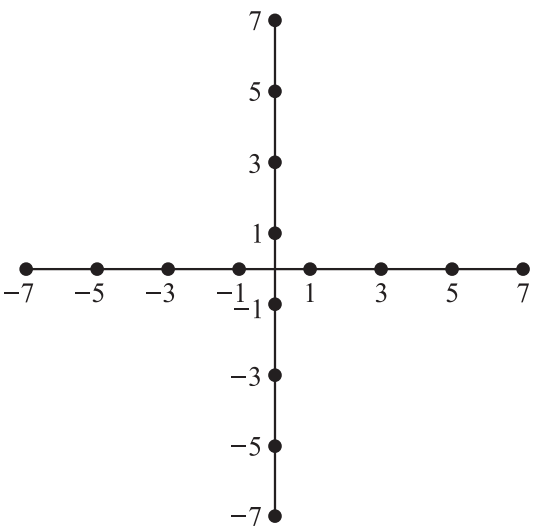
\includegraphics[scale=0.6]{HW2-1-1.png}
            	\caption{QAM signal constellation}
            % 	\label{fig}
            \end{figure}
    %%%%%%%%%%%%%%%%%%%%%%%%%%%%%%
        \item
            Consider a digital communication system that transmits information via QAM over a voice-band telephone channel at a rate of $2400$ symbols/s. The additive noise is assumed to be white and Gaussian. \\
            (a) Determine the $\varepsilon_b / N_0$ required to achieve an error probability of $10^{-5}$ at $4800$ bits/s. \\ 
            (b) Repeat part (a) for a rate of $9600$ bits/s. \\ 
            (c) Repeat part (a) for a rate of $19,200$ bits/s. \\ 
            (d) What conclusions do you reach from these results? \\ 
    %%%%%%%%%%%%%%%%%%%%%%%%%%%%%%
        \item
            Let $X$ be a geometrically distributed random variable, i.e., $$P(X = k) = p(1-p)^{k - 1}, k = 1, 2, 3, ...$$
            (a) Find the entropy of $X$. \\ 
            (b) Given that $X > K$, where $K$ is a positive integer, what is the entropy of $X$? \\
            \newpage
    %%%%%%%%%%%%%%%%%%%%%%%%%%%%%    
        \item 
            A DMS has an alphabet of eight letters $\; x_i, \ i = 1, 2,..., 8,$ with probabilities $\ 0.25$, $0.20$, $0.15$, $0.12$, $0.10$, $0.08$, $0.05$, and $0.05$. \\
            (a) Use the Huffman encoding procedure to determine a binary code for the source output. \\ 
            (b) Determine the average number $\Bar{R}$ of binary digits per source letter. \\ 
            (c) Determine the entropy of the source and compare it with $\Bar{R}$. \\ 
    %%%%%%%%%%%%%%%%%%%%%%%%%%%%%%%%%%%%%%%%%%%%%%    
        \item 
            A discrete memoryless source has an alphabet of size 7, $\mathcal{X} = \{ x_1, \ x_2, \ x_3, \ x_4, \ x_5, \ x_6, \ x_7 \}$, with corresponding probabilities $\{ 0.02, \ 0.11, \ 0.07, \ 0.21, \ 0.15, \ 0.19, \ 0.25 \}$. \\
            (a) Determine the entropy of this source. \\ 
            (b) Design a Huffman code for this source, and find the average codeword length of the Huffman code. \\ 
            (c) A new source $\mathcal{Y} = \{ y_1, \ y_2, \ y_3 \}$ is obtained by grouping the outputs of the source $\mathcal{X}$ as 
            % $ y_1 = \{ x1, \ x2, \ x5 \}, \; y_2 = \{ x3, \ x7 \}, \; y_3 = \{ x4, \ x6 \}$ 
            $$ 
            \begin{aligned}
                & y_1 = \{ x1, \ x2, \ x5 \} \\
                & y_2 = \{ x3, \ x7 \} \\ 
                & y_3 = \{ x4, \ x6 \} \\
            \end{aligned}
            $$ \\
            Determine the entropy of $\mathcal{Y}$. \\
            (d) Which source is more predictable, $\mathcal{X}$ or $\mathcal{Y}$ ? Why? \\ 
    %%%%%%%%%%%%%%%%%%%%%%%%%%%%%%
        \item 
            A memoryless source has the alphabet $A = \{-5, \ -3, \ -1, \ 0, \ 1, \ 3, \ 5 \}$, with corresponding probabilities $\{ 0.05, \ 0.1, \ 0.1, \ 0.15, \ 0.05, \ 0.25, \ 0.3 \}$. \\ 
            (a) Find the entropy of the source. \\ 
            (b) Assuming that the source is quantized according to the quantization rule
            $$\left\{ 
            \begin{aligned}
                & q(-5) = q(-3) = -4 \\
                & q(-1) = q(0) = q(1) = 0 \\ 
                & q(3) = q(5) = 4 \\
            \end{aligned}
            \right.
            $$ \\
            find the entropy of the quantized source.
            % \newpage
    %%%%%%%%%%%%%%%%%%%%%%%%%%%%%%%%%%%%%%%%%%%%%%
    \end{enumerate}
    \rule{\textwidth}{0.4pt}
\end{document}


